%
% main.tex -- Paper zum Thema <antennen>
%
% (c) 2020 Autor, OST Ostschweizer Fachhochschule
%
% !TEX root = ../../buch.tex
% !TEX encoding = UTF-8
%
\chapter{Thema\label{chapter:antennen}}
\kopflinks{Thema}
\begin{refsection}
\chapterauthor{Baris Catan und Jannis Gull}

Das Ziel dieses Kapitels ist, den Wirkungsgrad einer Loop-Antenne mittels Formoptimierung zu erhöhen. Für die Umsetzung dieser Problemstellung wird eine direkte Methode der Variation, in diesem Fall das Verfahren nach Ritz, verwendet.

Nach einer Übersicht über die physikalischen Eigenschaften von Loop-Antennen wird die zu optimierende Form vorgestellt. Nach einer Einführung über das Verfahren nach Ritz kann dieses gleich angewendet werden und eine optimale Antennenform bestimmt.

%
% antennenAllgemein.tex 
%
% 
%
% !TEX root = ../../buch.tex
% !TEX encoding = UTF-8
%

\section{Antennen\label{antennen:antennenAllgemein}}
\kopfrechts{Antennen}
Antennen sind in der heutigen technologischen Welt unverzichtbar.
Sie sind in zahlreichen Formen und Varianten in fast allen
elektronischen Geräten zu finden. Ihre primäre Funktion besteht
darin, elektromagnetische Wellen von einer leitungsgebundenen Form
\index{elektromagnetische Wellen}%
\index{Wellen, elektromagnetische}%
in freie Wellen im Raum zu verwandeln. Dieser Vorgang ist essenziell
für die Kommunikation, da er die Übertragung von Signalen über große
Distanzen ermöglicht. Ein weiterer entscheidender Aspekt von Antennen
ist ihre Reziprozität: Sie können sowohl Signale senden als auch
\index{Reziprozität}%
empfangen. Dabei wandeln sie freie Wellen aus dem Raum zurück in
leitungsgebundene Wellen. Diese Fähigkeit macht Antennen zu einem
grundlegenden Element der modernen Kommunikationstechnologie. Ohne
sie wäre die drahtlose Übertragung von Daten und Signalen, wie wir
sie heute kennen, undenkbar.

Eine genauere Erklärung von elektromagnetischen Wechselwirkungen findet der Leser im Kapitel \ref{chapter:maxwell},
welches sich mit den Maxwell-Gleichungen befasst. 
\index{Maxwell-Gleichungen}%

\subsection{Loop-Antennen\label{antennen:antennenAllgemein_loop}}


Eine Loop-Antenne hat eine recht simple Funktionsweise. Sie besteht aus einem Stück Draht wie in Abbildung \ref{antennen:loopAntenne} dargestellt. Die Loop-Antenne kann, nicht wie der Name impliziert, verschiedenste Formen annehmen. Durch den Leiter wird ein Signal geführt, das in der aufgespannten Fläche ein magnetisches Feld induziert. Dieses Feld wird durch Anpassung der Signalamplitude verändert. Eine solche Änderung kann als Information angesehen werden, die sich nun im freien Raum fortbewegt.

\begin{figure}
	\centering
	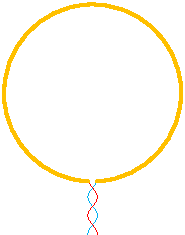
\includegraphics{papers/antennen/images/loopAntenne.pdf}
	\caption{Form einer typischen Loop-Antenne}
	\label{antennen:loopAntenne}
\end{figure}

\subsection{Eigenschaften\label{antennen:antennenEigenschaften}}
Der Wirkungsgrad
\index{Wirkungsgrad}%
\begin{equation}
	\eta=\frac{P\textsubscript{rad}}{P\textsubscript{tot}},
	\label{antennen:Wirkungsgrad}
\end{equation}
auch Effizienz genannt, kann mittels der eingespeisten Gesamtleistung
der Antenne $P\textsubscript{tot}$ und der abgestrahlten Leistung
$P\textsubscript{rad}$ berechnet werden. Eine Leistung $P$ entspricht
dem elektrischen Widerstand multipliziert mit der Stromstärke im
Quadrat. Nach Vereinfachung ergibt sich, dass die Effizienz
\begin{equation}
	\eta=\frac{P\textsubscript{rad}}{P\textsubscript{tot}}=\frac{R\textsubscript{rad}\cdot{I^2}}{R\textsubscript{tot}\cdot{I^2}}=\frac{R\textsubscript{rad}\cdot{I^2}}{(R\textsubscript{rad}+R\textsubscript{loss})\cdot{I^2}}=\frac{R\textsubscript{rad}}{R\textsubscript{rad}+R\textsubscript{loss}}
	\label{antennen:Wirkungsgradkomplett}
\end{equation}
nur noch vom Verlustwiderstand und dem Strahlungswiderstand abhängig ist. $R\textsubscript{rad}$ und $R\textsubscript{loss}$ werden wie folgt definiert:
\index{Verlustwiderstand}%
\index{Strahlungswiderstand}%
\begin{align}
	R_{\text{rad}} &= 31171 \Omega \cdot \bigg( \frac{A}{\lambda^2} \bigg)^2 \tag{20.3} \label{antennen:Rrad} \\
	R_{\text{loss}} &= \frac{\rho \cdot l}{r^2 \cdot \pi}. \tag{20.4} \label{antennen:Rloss}
\end{align}

Die Formel \eqref{antennen:Rrad} für die Berechnung des
Strahlungswiderstands wurde aus Fachliteratur \cite{antennen:antennaTheory}
übernommen, welche erklärt, dass die ``magische'' Konstante in
\eqref{antennen:Rrad} durch elektrodynamische Gesetzte entsteht.
Sie gilt für die verschiedensten Formen von Loop-Antennen, welche
einen kleinen Umfang  $l$ < $\lambda$/10 aufweisen. $A$ wird hierbei
als aufgespannte Fläche definiert, während $\lambda$ der Wellenlänge
entspricht. Eine Wellenlänge
\setcounter{equation}{4}
\begin{equation}
	\lambda = \frac{c}{f}
	\label{antennen:lambda}
\end{equation}
entspricht dem Verhältnis der materialspezifischen Lichtgeschwindigkeit $c$ und der Einsatzfrequenz $f$.
\index{Lichtgeschwindigkeit}%
\index{c@$c$}%
Der Verlustwiderstand wird aus dem spezifischen Widerstand $\rho$, dem Umfang $l$ und dem Leiterradius $r$ berechnet. Die Formeln \eqref{antennen:Rrad} und \eqref{antennen:Rloss} können in dieser Arbeit vereinfacht werden, da die Einsatzfrequenz und die Drahteigenschaften als konstant und gegeben angesehen werden können. Es resultieren die Ausdrücke 
\begin{align}
	R_{\text{rad}} &= k_{\text{1}} \cdot A^2 \tag{20.6} \label{antennen:Rrad_konst} \\
	R_{\text{loss}} &= k_{\text{2}} \cdot l \tag{20.7} \label{antennen:Rloss_konst}
\end{align}
für die beiden Widerstände. $k\textsubscript{1}$ und $k\textsubscript{2}$ werden als Konstanten betrachtet. Eingesetzt in \eqref{antennen:Wirkungsgradkomplett} ergibt sich
\setcounter{equation}{7}
\begin{equation}
\eta
=
\frac{
k\textsubscript{1}\cdot{A^2}
}{
k\textsubscript{1}\cdot{A^2}+{k\textsubscript{2}\cdot{l}}
}
=
\frac{1}{
1+\displaystyle\frac{k\textsubscript{2}\cdot{l}}{k\textsubscript{1}\cdot{A^2}}
}
	\label{antennen:Wirkungsgradeingesetzt}
\end{equation}
für den Wirkungsgrad.

%%
% problemstellung.tex 
%
% 
%
% !TEX root = ../../buch.tex
% !TEX encoding = UTF-8
%

\section{Problem\label{antennen:problemstellung}}
\rhead{Problem}

bla bla antennen

knknknkn

kjkjkj
%
% unserRitz.tex 
%
% 
%
% !TEX root = ../../buch.tex
% !TEX encoding = UTF-8
%

\section{Das Ritz-Verfahren\label{antennen:ritzGrundsätzlich}}

Wie schon sehr oft in diesem Buch erwähnt, gibt es das Problem, dass man für ein Funktional
\begin{equation}
I(y)
=
\int_{x_1}^{x_2}L(x,y(x),y'(x))\,dx
\label{antennen:normalesFunktional}
\end{equation}
eine Funktion $y(x)$ finden muss, welche das Funktional extremal macht.
Solch eine Funktion ist die Lösung der Euler-Lagrange Differentialgleichung
\begin{equation}
\frac{\partial L}{\partial y} - \frac{d}{dx} \left( \frac{\partial L}{\partial y'} \right) = 0.
\label{antennen:el-DGL}
\end{equation}
Wenn diese Gleichung \eqref{antennen:el-DGL} 
jedoch analytisch nicht lösbar ist, kommt das Verfahren nach Ritz ins Spiel.

\subsection{Approximationsfunktion nach Ritz\label{antennen:approxFunkt}}

Aus der Fourier-Theorie weiss man, dass
periodische Funktionen $f(t)$ als Linearkombination von anderen Funktionen, 
im Sinne der Fourierreihe als
%todo WHY SIND KLAMMERN GROSS? CHECKS NID
\begin{equation}
f(t)
=
\frac{a_0}{2}+\sum_{n=1}^{\infty}[a_n\cos(n \omega_f t )+b_n\sin(n \omega_f t)]
\label{antennen:fourier}
\end{equation}
beschrieben werden können.

Eine ähnliche Idee wird beim Verfahren nach Ritz angewendet.
Es wird eine Approximationsfunktion in der Form
\begin{equation}
y(x)=\sum_{k=1}^n a_k \psi_k(x)
\label{antennen:ritzFunkt}
\end{equation}
definiert. Die Funktionen $\psi_k(x)$ und Koeffizienten $a_k$, oder
wie in der Welt des Verfahrens nach Ritz,  
\em Koordinatenfunktionen $\psi_k(x)$ \em und \em Koordinaten \em $a_k$.
Im weiteren Verlauf jedoch behalten wir die intuitiveren, zuerst genannten Namen.

\subsection{Mögliche Approximationsfunktionen\label{antennen:approxBsp}}

Je nach Problemstellung gibt es bessere oder schlechtere Approximationsfunktionen.
Mögliche ausgeschriebene Funktionen können so aussehen:
\begin{equation}
	\begin{aligned}
		\text{Potenz-Entwicklung: }
		y(x)
		&=
		a_0+a_1 x+a_2 x^2+\cdots+a_n x^n \\
		\text{Fourier-Entwicklung: } 
		y(x)
		&=
		a_0+a_1\cos(x)+b_1\sin(x)+\cdots+a_n\cos(n x)+b_n\sin(n x)\\
		\text{Exponential-Entwicklung: } 
		y(x)
		&=
		a_1 e^{\lambda x}+a_2 e^{-\lambda x}+\cdots+a_n e^{(-1)^n \lambda}
	\end{aligned}
\label{antennen:approxFunktBsp}
\end{equation}

Das Ziel ist es schlussendlich, das Problem so genau wie nötig mit so wenig
Koeffizienten wie möglich auszudrücken.


%%
% resultat.tex 
%
% 
%
% !TEX root = ../../buch.tex
% !TEX encoding = UTF-8
%
%\usetikzlibrary{spy}
\section{Finale Überlegungen\label{antennen:resultat}}
\kopfrechts{Finale Überlegungen}
Das Kapitel \ref{antennen:ritzAnw} hat gezeigt, dass ein Abrundung an den Ecken
zur besten Effizienz führt, weil die abgerundete Form das Verhältnis \eqref{antennen:Verhältnis}
minimiert und somit die Effizienz maximiert. Wie gross der Radius dieser Abrundung
ist, muss jedoch noch bestimmt werden.


\subsection{Parametrisierung der abgerundeten Dreiecksantenne\label{antennen:param3eck}}
Die Länge $l$, hierbei der Umfang 
des abgerundeten Dreiecks, sowie dessen Fläche $A$ kann mit den Formeln
\definecolor{clrGreen}{RGB}{0, 117, 18}
\definecolor{drkOrange}{RGB}{255, 130, 28}
\begin{align}
	l &= \textcolor{blue}{2 \cdot \pi \cdot r} + \textcolor{drkOrange}{3 \cdot s - 6 \cdot \sqrt{3} \cdot r} \tag{20.24} \label{antennen:Länge} \\
	A &= \textcolor{clrGreen}{r^2 \cdot \pi} + \textcolor{black}{3 \cdot r \cdot (s - 2 \cdot \sqrt{3} \cdot r)} + \textcolor{darkred}{\frac{\sqrt{3} \cdot (s - 2 \cdot \sqrt{3} \cdot r)^2}{4}} \tag{20.25} \label{antennen:Fläche}
\end{align}\setcounter{equation}{25}%
berechnet werden.
Der Wirkungsgrad ist nun zu einem eindimensionalen Problem mit zwei Variablen geworden, das nur noch abhängig von 
der Seitenlänge $s$ des Dreiecks und des Radius $r$ der Kreise ist. Bildlich ist dies 
in Abbildung \ref{antennen:tikzdreieckAufteilung} veranschaulicht.
\begin{figure}
	\centering
	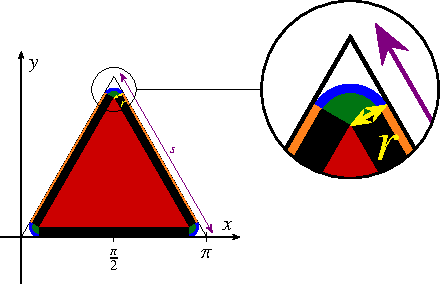
\includegraphics{papers/antennen/images/aufteilungDreieckZoom.pdf}
	\caption{Aufteilung des Dreiecks mit Zoom auf eine Ecke.}
	\label{antennen:tikzdreieckAufteilung}
\end{figure}

Durch Ableiten und Null setzten
\begin{equation}
	\frac{\partial}{\partial{r}} \bigg(\frac{l}{A^2}\bigg)=0
	\label{antennen:Ableitung}
\end{equation}
ergibt sich für eine gewünschte Seitenlänge $s$ ein Radius $r$ als Lösung. 
Die Ableitung ergibt die Gleichung 
\begin{equation}
	\frac{(- 4 \pi r + 12 \sqrt{3} r) (- 6 \sqrt{3} r + 2 \pi r + 3 s)}{\left(\pi r^{2} + 3 r (- 2 \sqrt{3} r + s) + \frac{\sqrt{3} \left(- 2 \sqrt{3} r + s\right)^{2}}{4}\right)^{3}} + \frac{- 6 \sqrt{3} + 2 \pi}{\left(\pi r^{2} + 3 r (- 2 \sqrt{3} r + s) + \frac{\sqrt{3} \left(- 2 \sqrt{3} r + s\right)^{2}}{4}\right)^{2}}=0.
	\label{antennen:Ableitunggelöst}
\end{equation}
Das Gleichungssystem hat hohen Grad. Die Lösung erfolgt numerisch, 
wobei es eine Herausforderung darstellt, mögliche und unmögliche Ergebnisse voneinander zu unterscheiden.

Als konkretes Beispiel wird der Parameter $s$, also die Seitenlänge des Dreiecks mit dem Wert $\pi$ definiert. 
Nach dem Lösen der Gleichung \eqref{antennen:Ableitunggelöst} mit dem Python-Skript \cite{antennen:codeAbleitung} erhält
man den Wert $r\approx0.2465$. Das Verhältnis zwischen Seitenlänge und Radius ist somit $\frac{\pi}{0.2465} \approx 12.744$.
Dieses Verhältnis kann nun für beliebige Seitenlängen verwendet werden und stellt somit eine wertvolle Hilfe für 
diejenigen dar, die eine optimale dreieckige Loop-Antenne entwerfen möchten.

\subsection{Fazit\label{antennen:fazit}}
In diesem Kapitel wurde eine dreieckige Antennenform ermittelt, welche die optimale Effizienz aufweist. Mittels dem Variationsprinzip von Ritz wurde dargelegt, dass eine Antenne in Form eines gleichseitigen Dreiecks für eine Effizienzsteigerung abgerundete Ecken benötigt. Das Verhältnis zwischen Seitenlänge und Radius $\frac{\pi}{0.2465} \approx 12.744$ ist optimal.



\printbibliography[heading=subbibliography]
\end{refsection}
